In the following experiments we evaluate the benefits of passing additional information through hypervisor layer to the  guests for detecting interference.  We first validate that our test infrastructure can accurately create I/O interference and we can measure that application throughput.  We find that the application throughput is dependent on the size of the test database.  Then we use our method to calculate the overhead on our \emph{Personal} size server.  We run two different sets experiments in this configuration to detect interference from both external memory pressure as well as external I/O.   Similarly we calculate the interference on our \emph{Business} size server, by adding one domain at a time.  These results show that our method can measure the interference from external systems and account for the performance drop in the application.  Our final test shows that our method does not report interference when our application is degraded from an application workload change.

\subsection{Validate Test Infrastructure}
In this experiment we verify that our test framework can generate a load that degrades the application when run with external interference.  We expect a significant drop in performance from running a single guest test to running multiple guests concurrently.  Monitoring resource counters in only the guest domain provides little information about external systems causing performance problems. 

\subsubsection{Without Interference}
For I/O intensive workloads, the application tends to perform very well when the entire \emph{working set} can fit into main memory, and the OS will cache reads from disk.  However, when the \emph{working set}  approaches (or exceeds) the size of main memory, the application tends to degrade quickly.  Our initial experiments to find an I/O workload highlight this fact by changing the database size under load in a virtual environment.  Before running the entire test suite we need to create a test database that will exceed the \emph{working set} and increase the probability that a database read will need to fetch the data from disk storage.  With PGbench the "-i" flag \emph{scaling factor} is used to initialize a database at a specified size (prior to running the benchmark) so that our results can show changes between a memory bound system and I/O bound system.  

To begin this exercise, we divide the physical memory and CPUs into four equal parts and create four individual guest virtual machines (Dom1 - Dom4).  
Each virtual machine is given an equal share of the memory and CPU resources so that no guest virtual machine would interfere with another machine if they were on separate physical systems.  
We start only our Dom1 machine and run our experimental test with PGbench.  
On our \emph{Business} size server, Dom1 is allocated 2GB vRAM and 2 vCPU, while on our \emph{Personal} server Dom1 is given 512MB vRAM and 1 vCPU.  

The test starts by initializing a very small database and runs PGBench and collect the TPS.  
Then we increase the DB size slightly and run the benchmark again.  
After repeating this process several times, we can determine when the DB size changes to an I/O bound system its performance drops significantly (Figure \ref{smallIO}).  
This is due to the fact that it must fetch database rows from the disk and it is much slower.  

\begin{figure}[!h]
  \begin{center}
  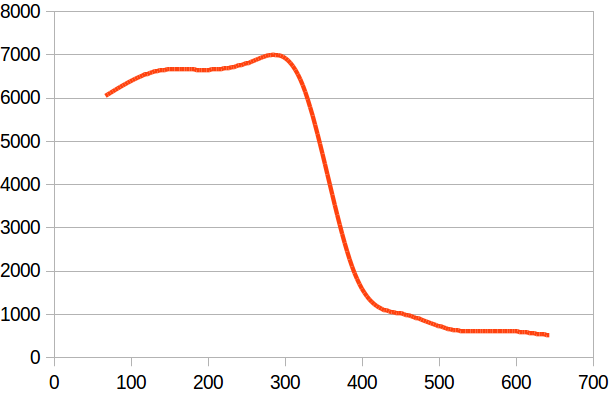
\includegraphics[width=4in]{images/SmallScale.png}
  \caption{TPS on our \emph{Personal} size server with 1 vCPU and 512KB vRAM. It changes from a memory bound application to an I/O bound application when the DB size approached the available RAM.}
  \label{smallIO}
  \end{center}
\end{figure}

From these tests we can now see the size of the database needed on each system to generate an I/O workload. 
\begin{description}
  \item[Small DB] The working set can fit into main memory.  Performance is based on memory.
  \item[Medium DB] The working set is swapped to disk occasionally. Performance is moving from memory to I/O.
  \item[Large DB] Most reads need to go to disk.  Performance is based on Disk I/O.
\end{description}

% Section 7.1.2
\subsubsection{With Interference}
Then we create external machine interference by running Dom1 concurrently with Dom2, Dom3, and Dom4. Each of the Dom2 - Dom4 systems are configured the same as Dom1.  We create a Large 2GB database on each guest of the Dell, and a Large 1GB database on each guest of the IBM.  We run PGBench in a loop to continuously create I/O interference on each external guest machine (Dom2 - Dom4). Concurrently we run our benchmark, and collect performance statistics only from Dom-1.  When the system is not I/O bound (Small DB) there is about a 28\% drop in performance (4434 TPS - 3208 TPS) on the \emph{Personal} server and little change in the \emph{Business} server (Table \ref{fig:tps1}).  On both servers the guest becomes an I/O bound system quicker with external interference.

\begin{table}[h]
\begingroup
    \fontsize{10pt}{12pt}\selectfont
\begin{subtable}[h]{0.45\textwidth}
  \begin{tabular}{ l | r | r | r }
    DB Size & Single & Interference & Drop \\
    \hline
    Small & 4434 & 3208 & 28\% \\ \hline
    Medium & 2149 & 216 & 90\% \\ \hline
    Large & 260 & 197 & 24\% \\  \hline
    \hline
  \end{tabular}
\caption{Interference from \emph{Personal} size server with 2GB RAM:  Each Guest domain has 512MB Allocated.}
\end{subtable}
\hfill
\begin{subtable}[h]{0.45\textwidth}
  \begin{tabular}{ l | r | r | r }
    DB Size & Single & Interference & Drop \\
    \hline
    Small & 5772 & 5734 & 0.7\% \\ \hline
    Medium & 1608 & 162 & 90\% \\ \hline
    Large & 359 & 82 & 77\% \\  \hline
    \hline
  \end{tabular}
\caption{\emph{Business} size server with 12GB RAM:  Each Guest domain has 2GB Allocated. }
\end{subtable}
\caption{Dom1 TPS difference from interference for 3 database sizes.}
\label{fig:tps1}
\endgroup
\end{table}

% Section 7.1.3
\begin{figure}[!h]
  \begin{center}
  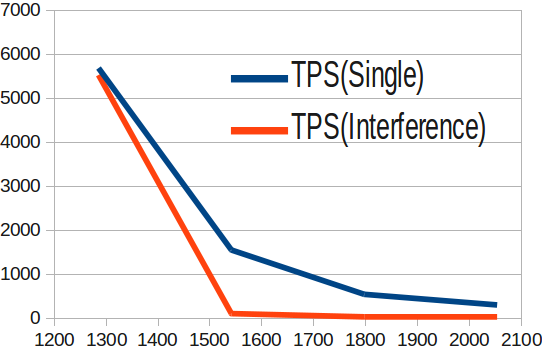
\includegraphics[width=4in]{images/MedScale.png}
  \caption{Application performance in transactions per second is degraded with interference.}
  \label{fig:medIO}
  \end{center}
\end{figure}

Trying to analyze the performance drop in Dom1 without knowing about this external interference is difficult.  There were no changes to Dom1 when run by itself and run with other guests.  By using the system \emph{vmstat} utility we can examine available memory, SwapIn and BytesIn/s to see if we can determine why the application benchmark is degraded without collecting external information (Figure \ref{fig:vmstat}).  Memory is not used as efficiently, the system almost completely eliminates swapping data in, and also does not read as much data from disk.  However, there is no indication that the problem was due to an external guest and hypervisor using those resources.  A DBA looking at these numbers may conclude that kernel swap or DB tuning may fix the problem.  
The root cause of the performance drop is due to external interference, which is not known from examining the data available.

\begin{table}[h]
  \begin{tabular}{ l | r | r | r }
    VMstat & Single & Multiple & Drop \\ \hline
	SwapIn/s & 1,480 & 85 & 94\% \\
	BytesIn/s & 6,877 & 4,438 & 35\% \\
	CPU IOwait & 92\% & 93\% & 1\% \\
  \end{tabular}
\caption{Statistics using performance tool \emph{vmstat} on guest Dom1 with a Large database while running alone and with external interference.} 
\label{fig:vmstat}
\end{table}

% Section 7.2
\subsection{Personal Server}
In the previous experiment we showed the interference that can occur when external I/O interference is applied to a guest domain, and only looking at the performance counters in the guest does not indicate the problem.  In this experiment, we verify our design to measure interference from external systems, when the system is I/O bound.  The results are from our IBM x3650, where each guest is configured to use 512MB of vRAM.  First, we run the benchmark with a large 640MB database without interference and calculate the overhead.  Then we start Dom2 - Dom4, while running the benchmark in Dom1, and calculate the interference.  We compare the results of the calculated interference with the performance drop in the application.  In all of these results we show the average of at least three test runs.

%\begingroup
%    \fontsize{10pt}{12pt}\selectfont
\begin{Verbatim}
# xm list
Name                     ID   Mem VCPUs      State  Time(s)
Domain-0                  0  1988     4     r-----  88871.2
Test_VM1                  1   512     1     -b----  60187.0
Test_VM2                  2   512     1     -b----   5722.0
Test_VM3                  3   512     1     -b----   5273.0
Test_VM4                  4   512     1     -b----   5203.5
\end{Verbatim}
%\endgroup

% Section 7.2.1
\subsubsection{Overhead}
We calculate the overhead at $4.7\%$ using the resource counters defined in our design and Equation 3 \ref{tab:OverheadSmall}.  The guest (Dom0) needs to wait about $5\%$ longer than the physical writes take to complete.  While calculating the overhead we also collected the application performance at 415 TPS without any external interference.

% See Test7_1Results.xls (Barbaro - Exp7.2(P2))
\begin{table}[h]
\begin{tabular}{ l l l p{5cm} }
  Counter     & Dom0 & Dom1 & $Overhead_{IO}$ \\
  \hline
	pgpgin    & 332,504 & 165,901  &  \\
	pgfault   &  25,648 & 132,691  & \\
	r sectors & 332,504 & 331,803  &\\
	r\_ms     &  63,356 &  72,428  & \\
	r total   &  11,145 &  12,166  & \\
    \textbf{reads/s}    & 372 & 406 & \\
    \textbf{AvgRdWait}  & 5.68 & 5.95 & 4.7\% \\ 
  \hline
\end{tabular}
\caption{Overhead on the \emph{Personal} size server.}
\label{tab:OverheadSmall}
\end{table}

One thing to notice is that the \emph{pgpgin} (count of pages in using \emph{/proc/vmstat}) from the Dom0 is twice as much as Dom1.  We also see in Dom0 that pgpgin is exactly the same as the sectors read, while there is exactly twice as many read sectors in Dom1.
After much research reviewing the \emph{sar} man page \footnote{We also verified this by looking at the sar code and kernel code for virtual memory}, we found that the pgpgin is reporting 1 Kbyte pages.  The \emph{fdisk -l} command showed the sector size as 512 bytes per sector.  We verified this on physical hardware by examining the statistics while copying files.  There were 2 sectors read for each page in.  We also ran this test on only Dom0 and found the same results:  There were 2 sectors read per page in.  The expected results should be 2 read sectors for each page in, but when reading from Dom1, Dom0 always showed a 1:1 ratio.

After closer examination of the method used to pass reads with Xen, we found that there is an additional block device in Dom0 \cite{citrix}.  Although this does not map to a physical device it does explain the strange \emph{pgpgin} between Dom0 and Dom1.  In the virtual guest (Dom1), when it reads from a virtual disk it uses the blkfront driver.  This communicates with the blkback driver in Dom0.  There is an additional virtual disk in Dom0 used to pool requests.  Although this is not a physical device it still uses the virtual memory of the kernel and pages in for Dom0.  So each read sector (from physical disk) in Dom0 results in 2 pages in which is exactly what our data shows.

This additional work in Dom0 is an example of the overhead from virtualization, and partially explains the additional wait time in the guest.  We measure the additional time time waiting in the guest domain to account for all of the overhead the hypervisor must do in order to virtualize the physical device.

% Section 7.2.2 - Test7_1Resultx.xls (Barabaro- Exp7.2(P2))
\subsubsection{Memory Interference}
We repeat the previous experiment with 4 guest domains all running at the same time.  Since the DB size in Dom1 is 640MB and there is 512MB of vRAM on Dom1, we can say that Dom1 is bound by disk I/O speed.  We run the experiments with the other 3 guest domains running a memory bound database.  We create a Small DB of 128MB in each of the external domains to generate memory interference on Dom1.

\begin{table}[h]
\begin{tabular}{ l l l l p{5cm} }
  Counter & Dom0 & Dom1 & $Interference_{RPS}$ \\
  \hline
	pgpgin    & 328,144 & 128,176 &  \\
	pgfault   &  57,293 &  95,591 &  \\
	r sectors & 328,144 & 256,352 &  \\
	r ms      & 103,483 &  70,751 &  \\
	r total   &  13,365 &   9,547 &  \\
    \textbf{reads/s}    & 446 & 318 & 28.6\%  \\
    \textbf{AvgRdWait}  & 7.74 & 7.41 & \\ 
  \hline
\end{tabular}
\caption{Calculated Interference with external interference from small database in Dom2 - Dom4.  TPS dropped by 20\%} 
\label{fig:InterferenceSm}
\end{table}
We also need to calculate the increased wait time using the wait time $AvgRdWait$ in the hypervisor without interference ($5.68 ms$) and the new wait time in the hypervisor ($7.74 ms$). We calculate $Interference_{ARW} = 26.6\%$ (Equation 5).  Since this is slightly less than the interference from reads per second ($28.6\%$) we calculate the $Interference_{EXT} = 26.6\%$.

From these tests, Dom1 had 331 TPS, and was degraded from 415 TPS, a performance drop in the application of 20\%.  It is not shown in these results, but Dom2 - Dom4 was able to cache the entire working set in memory and did not issue any read requests.  Dom1 was the only domain to issue read request, but there was additional read time in the guests and hypervisor. 

% Section 7.2.3 - Test7_1Resultx.xls (Barabaro- Exp7.2(P2))
\subsubsection{I/O Interference}
Now we create I/O interference in the three guest domains by creating a 640MB Large DB in Dom2 - Dom4.  Since each guest has 512MB vRAM, this should cause significant I/O contention in Dom1.

\begin{table}[h]
\begin{tabular}{ l l l l p{5cm} }
  Counter     & Dom0    & Dom1    & $Interference_{RPS}$ \\
  \hline
	pgpgin    & 549,419 & 97,092 &  \\
	pgfault   &  58,201 & 86,765 &  \\
	r sectors & 549,419 &194,163 &  \\
	r ms      & 285,334 & 71,585 &  \\
	r total   &  20,723 &  7,259 &  \\
    \textbf{reads/s}    & 691 & 242 &   65\% \\
    \textbf{AvgRdWait}  & 13.8 & 9.86 &  \\ 
  \hline
\end{tabular}
\caption{Interference calculated Large 640MB DB in Dom2 - Dom4.  TPS dropped by 39\%}
\label{fig:InterferenceLg}
\end{table}
We also need to calculate the additional wait time in the hypervisor (Equation 5).  Without interference the read wait time is $5.68 ms$ and with interference it is $13.8 ms$.  We calculate $Interference_{ARW} = 58.7\%$  Since this is less than the interference from throughput we calculate the $Interference_{EXT} = 58.7\%$.

During these tests, the application benchmark in Dom1 decreased to 254 TPS.  This is much less than when run without interference (415 TPS) and with memory interference (331 TPS).  All of the read counters showed significant interference.  Additionally we are showing some interference from page faults.  

\subsubsection{Results Analysis}

% Test7_1Results.xls Barbaro-Exp7.2(P2)
\begin{figure}[!h]
  \begin{center}
  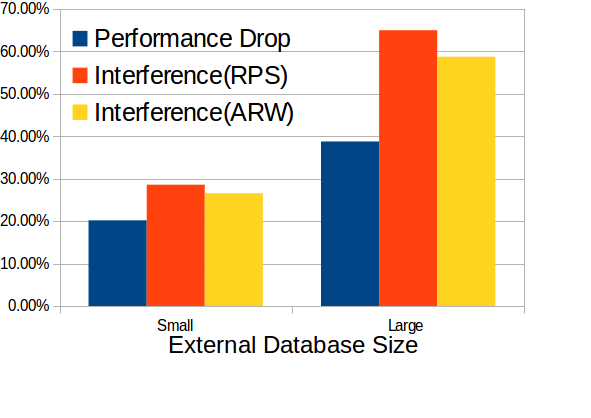
\includegraphics[width=4in]{images/IBM_PerfDrop_Int.png}
  \caption{Application performance drop compared to calculated interference, for two types of external interference.}
  \label{fig:perfDrop}
  \end{center}
\end{figure}

In both cases (Figure \ref{fig:perfDrop}) we calculate a higher interference than the application degrades.  At a minimum this implies that there is interference to the guest application.  Although the database is I/O bound there is still a percentage of the application that relies on the CPU speed which is not part of the interference.  

% 4.3 Section - Dell T410
\subsection{Business Server}
For this experiment we use our Dell T410 server with 12GB of physical RAM. We configure all Dom1 to use 4GB of vRAM and configure Dom2 - Dom4 as noted below.  We assign some different CPUs to the guest machines. We create a medium database of 3.2GB in Dom1.   And create Medium and Large databases in the external guest domains create different workloads in the guests.

\begin{Verbatim}
Name                       ID   Mem VCPUs      State   Time(s)
Domain-0                    0   872    16     r-----  27116.4
TestVM1                     1  4096     1     -b----   1127.7
TestVM2                     2  3072     2     -b----   1735.8
TestVM3                     3  2048     1     -b----   1588.1
TestVM4                     4  2048     2     -b----   1906.1
\end{Verbatim}

\subsubsection{Overhead}
We calculate the $Overhead_{IO}$ in Dom1 using equation 3.  The overhead from virtualization on this platform (2.4\%).   When comparing the these results on this size platform to the overhead in the previous size platform \ref{tab:OverheadSmall} we can see that our reads/s  decreased, but our database throughput is faster at 1,348 TPS.  In this server the database size is slightly smaller than the available memory (Table \ref{tab:OverheadDell}).

\begin{table}[h]
\begin{tabular}{ l l l p{5cm} }
  Counter     & Dom0 & Dom1 & $Overhead_{IO}$ \\
  \hline
    \textbf{reads/s}    & 275  & 281 & \\
    \textbf{AvgRdWait}  & 13.6 & 13.9 & 2.4\% \\ 
  \hline
\end{tabular}
\caption{Overhead on the \emph{Business} size server.}
\label{tab:OverheadDell}
\end{table}

\subsubsection{Interference}
% See WallEve_4_16_14.txt 
In the previous experiment for calculating interference we used 3 external guest domains, and changed the workload in the guest domains.  In this experiment, we create interference adding 1 external domain at a time.  The first result is a single guest domain Dom1 without external interference.  Then we run Dom1 with Dom2 and calculate the interference with one external domain.  We continue to add guest domains and calculate the interference and application performance drop in TPS (Table \ref{tab:domains}).

\begin{table}[!h]
\begin{tabular}{ l l l l l l p{2cm} }
                   & TPS   & reads/s & reads/s & AvgRdWait & $Inter_{RPS}$ & $Inter_{AWR}$ \\
	Experiment     & Dom 1 & Dom0     & Dom1     & Dom0      & $Inter_{EXT}$ &             \\
	\hline
    Dom1 (Only)     &1,348 & 275      & 281      & 13.6     &  -2.1\%  &   0.0\%   \\
    Dom1 + 1 guest  &  703 & 214      & 137      & 33.2     &  35.8\%  &   56.0\%  \\
    Dom1 + 2 guests &  543 & 246      & 108      & 44.0     &  56.1\%  &   67.1\%    \\
    Dom1 + 3 guests &  378 & 259      &  76      & 59.5     &  70.6\%  &   77.2\%  \\
\end{tabular}
\caption{Interference generated from 0, 1, 2, and 3 external guest domains.}
\label{tab:domains}
\end{table}

By examining these results as more external domains are added, the application TPS performance degrades as expected.  We are also able to measure the interference which increases as more domains are added.  The interference increases similar to the rate at which domains are added and the performance drop.

\subsubsection{Results Analysis}
First we examine the results of three tests in each configuration with external interference.  In this test we can see how the calculated interference relates to the performance drop in each experiment.  As more domains are added, the application performance drop increases similar to the measured interference (Figure \ref{fig:perfDropDell}).

% Test7_1Results.xls 7.3(Deux)
\begin{figure}[!h]
  \begin{center}
  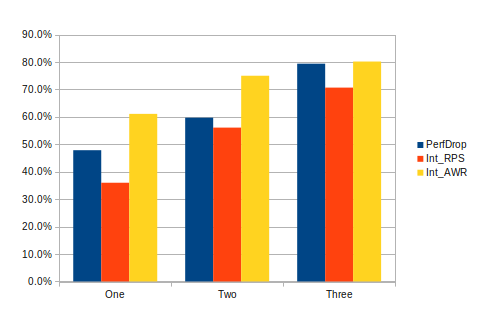
\includegraphics[width=4in]{images/Dell_PerfDrop_Int.png}
  \caption{\emph{Business} size application performance drop compared to calculated interference, for one, two and three external domains.}
  \label{fig:perfDropDell}
  \end{center}
\end{figure}

\subsubsection{Statistical Analysis}
In the previous experiments, we only had a sample size of 3 runs.  Although each run was for 30 seconds, we need to see how each run changes.  Now we run this experiment 30 times in each configuration to see how much change is occurring in each test.  We receive similar results as when only with 3 tests, but we can see that the standard deviation increases in both our application measurement and measured interference as more external domains are added (Table \ref{tab:stats}) (Figure \ref{fig:stats1}).

\begin{table}[!h]
\begin{tabular}{ l l l l p{3cm} }
	Experiment  & TPS        & reads/s  & AvgRdWait   & $Inter_{RPS}$ \\ 
	\hline
    Dom1 (Only)     &1,247 (55)  & 317 (15.9) & 14.7 (0.5)  &  N/A   \\
    Dom1 + 1 guest  & 585 (28)   & 163 (8.3)  & 37.3 (2.1)  & 36.6\% (3.3\%)  \\
    Dom1 + 2 guests & 537 (43)   & 148 (12.3) & 43.1 (5.0)  & 40.9\% (4.6\%) \\
    Dom1 + 3 guests & 430 (61)   & 118 (16.5) & 55.6 (9.7)  & 51.8\% (5.8\%) \\
\end{tabular}
\caption{Mean (Standard Deviation) from 30 runs of 0, 1, 2, and 3 external guest domains.}
\label{tab:stats}
\end{table}

% Stats_30runs.ods
\begin{figure}[!h]
        \centering
        \begin{subfigure}[b]{0.3\textwidth}
                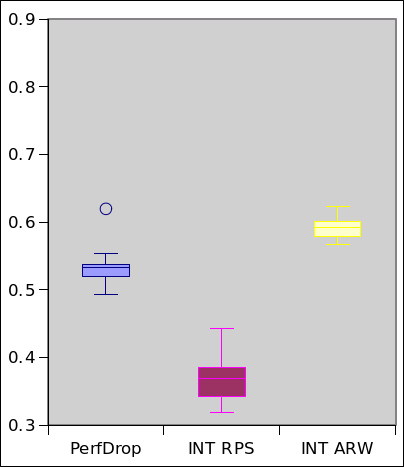
\includegraphics[width=\textwidth]{images/stats2Guest.png}
                \caption{1 external domain}
  		\label{fig:box2}
        \end{subfigure}%
         %add desired spacing between images, e. g. ~, \quad, \qquad, \hfill etc.
         %(or a blank line to force the subfigure onto a new line)
        \begin{subfigure}[b]{0.3\textwidth}
                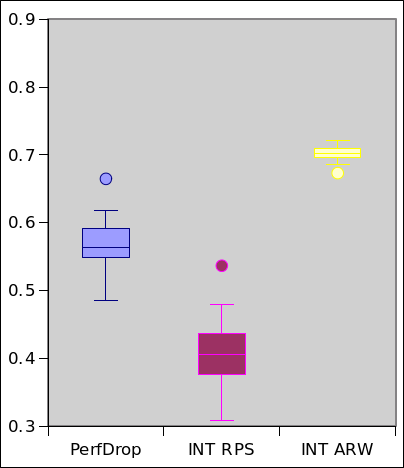
\includegraphics[width=\textwidth]{images/stats3Guest.png}
                \caption{2 external domains}
                \label{fig:box3}
        \end{subfigure}
         %add desired spacing between images, e. g. ~, \quad, \qquad, \hfill etc.
         %(or a blank line to force the subfigure onto a new line)
        \begin{subfigure}[b]{0.3\textwidth}
                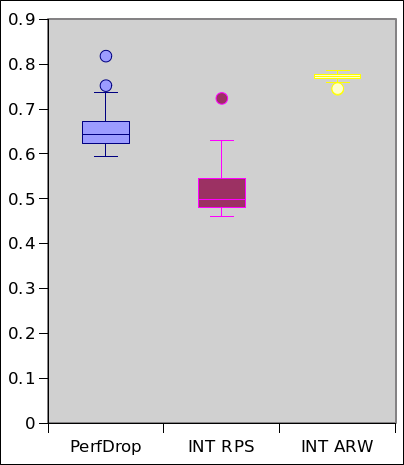
\includegraphics[width=\textwidth]{images/stats4Guest.png}
                \caption{3 external domains}
                \label{fig:box4}
        \end{subfigure}
  	\caption{Box plot with quartiles and outliers for application performance and calculated interference for 90 test runs.}        
	\label{fig:stats1}
\end{figure}

Finally, we need to show that the calculated interference relates to the application performance drop.  We use a linear regression over the 90 runs.  Although one and two external domains were similar, each test run would have different calculated interference and application performance.  We show that the calculated interference can explain the application performance drop (Figure \ref{fig:regression}).

% Stats_30runs.ods
\begin{figure}[!h]
  \begin{center}
  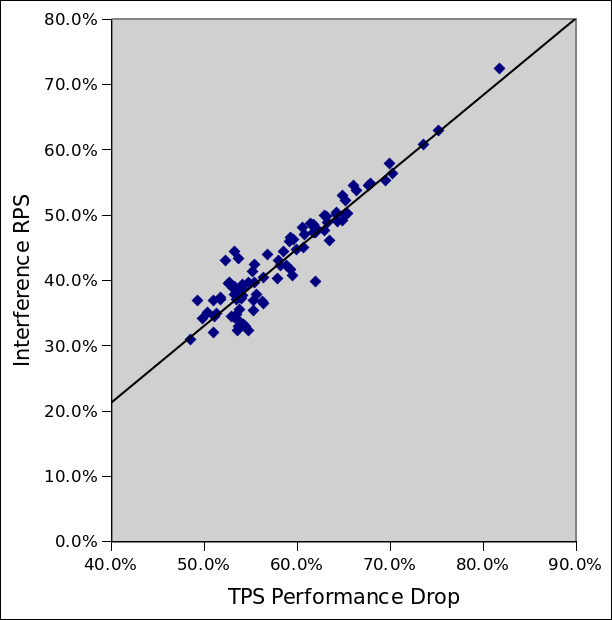
\includegraphics[width=4in]{images/scatterPlot.png}
  \caption{Linear regression of interference.  $R^2 = 0.8882$ }
  \label{fig:regression}
  \end{center}
\end{figure}


% Section 7.5
\subsection{Verification Without Interference}
In the previous two experiments, we showed how our method can give a guest domain vital information when it is degraded from external interference.  However, what if the guest domain was degraded due to an application bug, DB change, or misconfiguration?   In that case we want our method to show that there is not any external interference.

We have previously demonstrated that the database performance can become degraded as the size of the database increases.  Now we show that by simply increasing the size of the database, that our method does not report external interference.  In this case the application is degraded because the working set exceeds the available memory.  We also change the number of database connections to change the read wait time.  In either case, the application is not degraded due to external interference, and our method accurately indicates there is not any external interference.

% See Test7_1Results.xls - Barbaro Exp7.2 and Barbaro_Dom29.txt
\begin{table}[h]
\begingroup
    \fontsize{10pt}{12pt}\selectfont
\begin{tabular}{ l l l l l l p{9cm} }
                   & reads/s & reads/s & AvgRdWait & $Interfer_{RPS}$ & $Interfer_{AWR}$ \\
	Experiment     & Dom0     & Dom1     & Dom0      &                &             \\

    Test & Guest & Hypervisor  & $Interference_{RPS}$ \\
    \hline
    Baseline                   & 372 & 406 & 5.7 & -6\% & 0.0\%   \\  %Test 1
    Increase DB size           & 538 & 563 & 7.8 & -6\% & 26.9\% \\  %Test 3
    Increase DB Connections    & 836 & 875 &15.4 & -5\% & 63.0\% \\  %Test 4
	Decrease DB Connections    & 279 & 144 & 4.7 & 48\% & -17\%  \\  %Test 5
    With 3 ext domains         & 691 & 242 &13.8 & 65\% & 59.0\% \\  % From above
    \hline
  \end{tabular}
\caption{Tests without interference, our method does not report interference. }
\label{tab:HypervisorGuest}
\endgroup
\end{table}

One interesting result is that when we decreased the number of DB connections, we experienced a significant increase in reads in the hypervisor.  We ran this experiment several times, and verified that this was accurate.  For some reason the hypervisor increased the reads (since there were not any external domains).  Since our calculation determines interference from external domains, it did not show interference because there was no increase in the wait time.

By analyzing the throughput from both the guest layer and hypervisor layer, we can see that our method reports interference only when external interference is applied to the guest domain.  When we showed the guest view (Table \ref{tab:guestOnly}) it was difficult to determine if the problem was from a change in the guest application or an external domain.  With these tests we can see that we need to have both an increase in wait time in the hypervisor as well as additional throughput from external domains.


\subsection{Results Analysis}
We completed several different experiments on two different virtualization platforms.  In section 4.1 we verified our test method and showed how performance can decrease without interference by increasing the size of the database.  We also showed that for each database size when external guest domains run concurrently they cause interference and degrade the guest application.  In section 4.2 we looked at our \emph{Personal} size server which had 2 GB ram and 4 CPUs.  We were able to calculate the interference from external domains that only used memory, and external domains that were also I/O bound.  Our calculations for interference increased as the application performance decreased.  In section 4.3 we used our \emph{Business} server and calculated the overhead and interference from virtualization.  We created external interference from different numbers of guest domains, and found as more external guests are added our calculated interference increased similar to the application performance drop.  Finally, in section 4.4 we validated that when the application degrades due to internal changes, our method does not report it as external interference from virtualization.



